\documentclass[12pt,letterpaper]{article}
\usepackage[utf8]{inputenc}
\usepackage[spanish,english]{babel}
\usepackage{float, xcolor}

%----- Configuración del estilo del documento------%
\usepackage{graphicx, fancyhdr, lastpage}
\usepackage{enumitem, pifont}
\usepackage{multicol, tikz}

\usetikzlibrary{automata,arrows}
\usepackage[makeroom]{cancel}
\usepackage{changepage}
\usepackage{hyperref}
\usepackage[left=2cm,right=2cm,top=1.8cm,bottom=2.3cm]{geometry}

%------ Paquetes matemáticos básicos --------%
\usepackage{amsmath, amssymb, amsthm}

\newcommand{\M}{\mathcal{M}}
\newcommand{\imp}{\rightarrow}
\newcommand{\vp}{\varphi}
\newcommand{\dmp}{\leftarrow}

\begin{document}

%------ Encabezado -------- %
\hrule height 0.1pt
\bigskip

\begin{center}
  \begin{minipage}{3cm}
    \begin{center}
      
\includegraphics[height=3.4cm]{../unam_logo.png}
    \end{center}
  \end{minipage}\hfill
  \begin{minipage}{10cm}
    \begin{center}
      \textbf{\Large Universidad Nacional Autónoma de México}\\[0.2cm]
      \textbf{\large Facultad de Ciencias}\\[0.2cm]
      \textbf{Lógica Computacional | 2025-2}\\[0.4cm]
      \textbf{\Large Tarea 05}\\[0.1cm]
      \textbf{Docentes:}\\
      Noé Hernández \hspace{0.9em} Santiago Escamilla \hspace{0.9em} Ricardo López\\[0.3cm]
      \textbf{Autores:}\\
      Fernanda Ramírez Juárez \quad Ianluck Rojo Peña\\[0.3cm]
      \textbf{Fecha de entrega:} Domingo 25 de mayo de 2025
    \end{center}
  \end{minipage}\hfill
  \begin{minipage}{3cm}
    \begin{center}
      
\includegraphics[height=3.4cm]{../fc_logo.png}
    \end{center}
  \end{minipage}
\end{center}

\bigskip
\hrule height 0.1pt
\bigskip

%------ Notas sobre la resolución --------%
\section*{Notas sobre la resolución.}

\begin{quote}
  \textbf{Nota general:} Cada ejercicio fue resuelto en base, y tomando como referencia, las notas de clase lcNota12.pdf.
  
  Adem\'{a}s de las clases presenciales impartidas por el profesor y ayudantes, tanto para resolver dudas como las pistas y consejos dados
\end{quote}


\bigskip
\hrule height 0.1pt
\bigskip

\newpage

%------ Contenido -------- %
\section*{Resolución de Ejercicios.}

\begin{enumerate}

\item (1.5 pts.) Sea $\mathbb{P}$ el programa $P(a)\dmp$ y $G$ la cláusula meta $\dmp P(X)$. ¿Es la sustitución vacía una sustitución de respuesta correcta? Justifique su respuesta.
  % -- Respuesta --
  
  \medskip

  Recordemos que por la \textbf{Definición 1.4} \textit{(en resumen)}\textbf{:}
  
  "Dado un programa lógico $P$ y una cláusula meta $G$, una sustitución $\theta$ es una sustitución de respuesta correcta si: $P \vDash \forall (\neg G\theta )$ donde la cuantificación universal aplica sobre todas las variables libres de $\neg G\theta.$"
  
  Tenemos al programa $\mathbb{P}$ con el \'{u}nico hecho $P(a) \dmp$, y a $G$ la cl\'{a}usula meta $\dmp P(X)$. Por lo que, aplicar $\theta$ a $G$ dado que $\theta$ es vacía, no cambia nada, y nos queda $G \theta = \dmp P(X)$.

  
  Luego, consideremos que su negación ($\neg G \theta$) se cumple: $\neg G \theta = \neg(\dmp P(X)) = P(X)$, por ende tendriamos $\mathbb{P} \vDash \forall P(X)$. Sin embargo en el programa $\mathbb{P}$, solo sabemos que $P(a)$ es verdadero.

  Por otro lado, sabemos que, para ser una sustitución de respuesta correcta bajo la sustitución vacía, necesitaríamos que $P(X)$ fuera verdadero para todo $X$, $i.e.$ para cualquier valor que le asociemos a $X$. Pero si tenemos por ejemplo, $P(X)$ con $X = b$, entonces $P(b)$ no es derivables de $\mathbb{P}$ porque $\mathbb{P}$ solo afirma $P(a)$ y nada m\'{a}s.
  
  Por lo tanto, la sustitución vacía no es una sustitución de respuesta correcta, porque como ya mostramos $P \nvDash \forall P(X)$.
  \bigskip
  
\item (2 pts.) 
  \begin{itemize}
  \item Considere el siguiente programa lógico
    \[
    P(X) \leftarrow P(f(X))
    \]
    junto con la cláusula meta $\leftarrow P(a)$. ¿Qué pasará al usar la resolución SLD?

  \item Ahora, suponga que agregamos el hecho $P(f(f(a)))$. Conteste la misma pregunta.
  \end{itemize}
  % -- Respuesta --

  \medskip

  Usamos resolución SLD para el primer caso:
  \begin{center}
    \begin{enumerate}[label=\arabic*.]
    \item \( P(X) \dmp P(f(X)) \)
    \item \( \dmp P(a) \)    \hspace{7.35cm} cl\'{a}usula meta
    \item \( \dmp P(f(a)) \) \hspace{1.06cm} $[X := a]$ \hspace{1.16cm} tomando $P(X)$ \hspace{0.5cm} \textit{Res} (1, 2)
    \item \( \dmp P(f(f(a))) \) \hspace{0.49cm} $[X := f(a)]$ \hspace{0.59cm} tomando $P(X)$ \hspace{0.5cm} \textit{Res} (1, 3)
    \item \( \dmp P(f(f(f(a)))) \) \hspace{-0.039cm} $[X := f(f(a))]$ \hspace{-0.029cm} tomando $P(X)$ \hspace{0.5cm} \textit{Res} (1, 4)
      \[
      \hspace{-15cm}
      \begin{array}{c}
        \cdot \\[0.3em]
        \cdot \\[0.3em]
        \cdot
      \end{array}
      \]
    \end{enumerate}
  \end{center}

  Notemos que esto se sigue infinitamente:
  \[
  \dmp P(f(f(f(f(a)))))
  \]
  \[
  \dmp P(f(f(f(f(f(a))))))
  \]

  Nunca podremos llegar a la cl\'{a}usula vac\'{i}a dado que la \'{u}nica variable a la que podemos aplicar sustituci\'{o}n es $X$ en $P(X) \dmp P(f(X))$ y como $P(X)$ es un hecho \textit{(cl\'{a}sula de Horn unitaria positiva)} tras la aplicar resoluci\'{o}n con $\dmp P(a)$ (una cl\'{a}usula meta), nos queda $\dmp P(f(X))$ (otra cl\'{a}usula meta) con el valor que se le haya dado a $X$ en la sustituci\'{o}n. Y al volver a intentar resoluci\'{o}n SLD sucede lo mismo, no podemos unificar $\dmp P(f(X))$ con algun $\dmp P(a)$, $\dmp P(f(a))$, $\dmp P(f(f(a)))$, $\cdots$, por lo que entramos en un bucle infinito sin llegar a la cl\'{a}usula vac\'{i}a.

  Por lo tanto, no se puede resolver la consulta.\\

  Ahora continuamos con el segundo caso, agregando el hecho $P(f(f(a)))$, usamos resolución SLD:
  \begin{center}
    \begin{enumerate}[label=\arabic*.]
    \item \( P(X) \dmp P(f(X)) \)
    \item \( P(f(f(a))) \)
    \item \( \dmp P(a) \)    \hspace{7.35cm} cl\'{a}usula meta
    \item \( \dmp P(f(a)) \) \hspace{1.06cm} $[X := a]$ \hspace{1.16cm} tomando $P(X)$ \hspace{0.5cm} \textit{Res} (1, 3)
    \item \( \dmp P(f(f(a))) \) \hspace{0.49cm} $[X := f(a)]$ \hspace{0.59cm} tomando $P(X)$ \hspace{0.5cm} \textit{Res} (1, 4)
    \item \( \square \)  \hspace{4.66cm} tomando $P(f(f(a)))$ \hspace{0.5cm} \textit{Res} (2, 5)
    \end{enumerate}
  \end{center}

  Al agregar el hecho $P(f(f(a)))$, llegamos a la cl\'{a}usula vac\'{i}a y obtuvimos una refutaci\'{o}n SLD exitosamente.

  \newpage
  
\item (1.5 pts.) Considere el siguiente programa lógico:
  \[\arraycolsep=1.4pt\def\arraystretch{1.5}
  \begin{array}{lcl}
    A(x) &\leftarrow& B(x)\\
    B(x) &\leftarrow& E(x)\\
    L(karl,x) &\leftarrow& A(x)\\
    B(franz)&&\\
    E(hansi)&&
  \end{array}
  \]
  Dé una derivación SLD para la consulta $\leftarrow E(y), L(karl,y)$ que use la regla de cómputo que tome la literal más a la derecha, y la regla de búsqueda que analice las cláusulas de arriba a abajo.
  % -- Respuesta --

  \medskip

  Sea $P$ el programa lógico:
  \[\arraycolsep=1.4pt\def\arraystretch{1.5}
  \begin{array}{lcl}
    A(x) &\leftarrow& B(x)\\
    B(x) &\leftarrow& E(x)\\
    L(karl,x) &\leftarrow& A(x)\\
    B(franz)&&\\
    E(hansi)&&
  \end{array}
  \]

  Damos la siguiente derivación SLD para la consulta $\dmp E(y), L(karl,y)$:
  \begin{center}
    \begin{enumerate}[label=\arabic*.]
    \item \( A(x) \dmp B(x) \)
    \item \( B(x) \dmp E(x) \)
    \item \( L(karl,x) \dmp A(x) \)
    \item \( B(franz) \) 
    \item \( E(hansi) \) 
    \item \( \dmp E(y), L(karl,y) \) \hspace{7cm} consulta
    \item \( \dmp E(y), A(y) \) \hspace{0.7cm} $[x := y]$ \hspace{0.7cm} tomando \( L(karl,y)\) \hspace{0.9cm} \textit{Res} (3, 6)
    \item \( \dmp E(y), B(y) \) \hspace{0.7cm} $[x := y]$ \hspace{1.6cm} tomando \( A(y)\) \hspace{0.87cm} \textit{Res} (1, 7)
    \item \( \dmp E(y) \) \hspace{1.77cm} $[x := y]$ \hspace{1.6cm} tomando \( B(y)\) \hspace{0.86cm} \textit{Res} (2, 8)
    \item \( \square \) \hspace{2.85cm} $[y := hansi]$ \hspace{0cm} tomando \( E(hansi)\) \hspace{0.85cm} \textit{Res} (5, 9)
    \end{enumerate}
  \end{center}

  Dado que llegamos a la cláusula vacía la resolución fue exitosa y por lo tanto, tenemos una refutación para $\dmp E(y), Q(karl, y)$ bajo la sustitución $\theta = [x:= y, y := hansi]$.
  
  Como la resolución es correcta, concluimos que:
  \[
  P \vDash \forall \neg(\neg E(y) \lor \neg L(karl,y)) \theta
  \]
  
  de manera que $\theta$ es una sustitución de respuesta correcta y $E(y) \land L(karl, y)$ es verdadera para cualquier modelo de $P$.
  \bigskip
  
\item (2 pts.) Considere el siguiente programa lógico:
  \[
  \begin{array}{lll}
    P(Y) &\leftarrow& Q(X,Y),R(Y).\\
    P(X) &\leftarrow& Q(X,X).\\
    Q(X,X) &\leftarrow& S(X).\\
    R(b).\\
    S(a).\\
    S(b).\\
  \end{array}
  \]
  Dibuje el árbol SLD para la cláusula meta $\dmp P(X)$ si la regla de cómputo de \textsc{Prolog} es usada. ¿Cuál es la sustitución de respuesta correcta?
  % -- Respuesta --

  \medskip

  \begin{center}
    \hspace{-1.2cm} 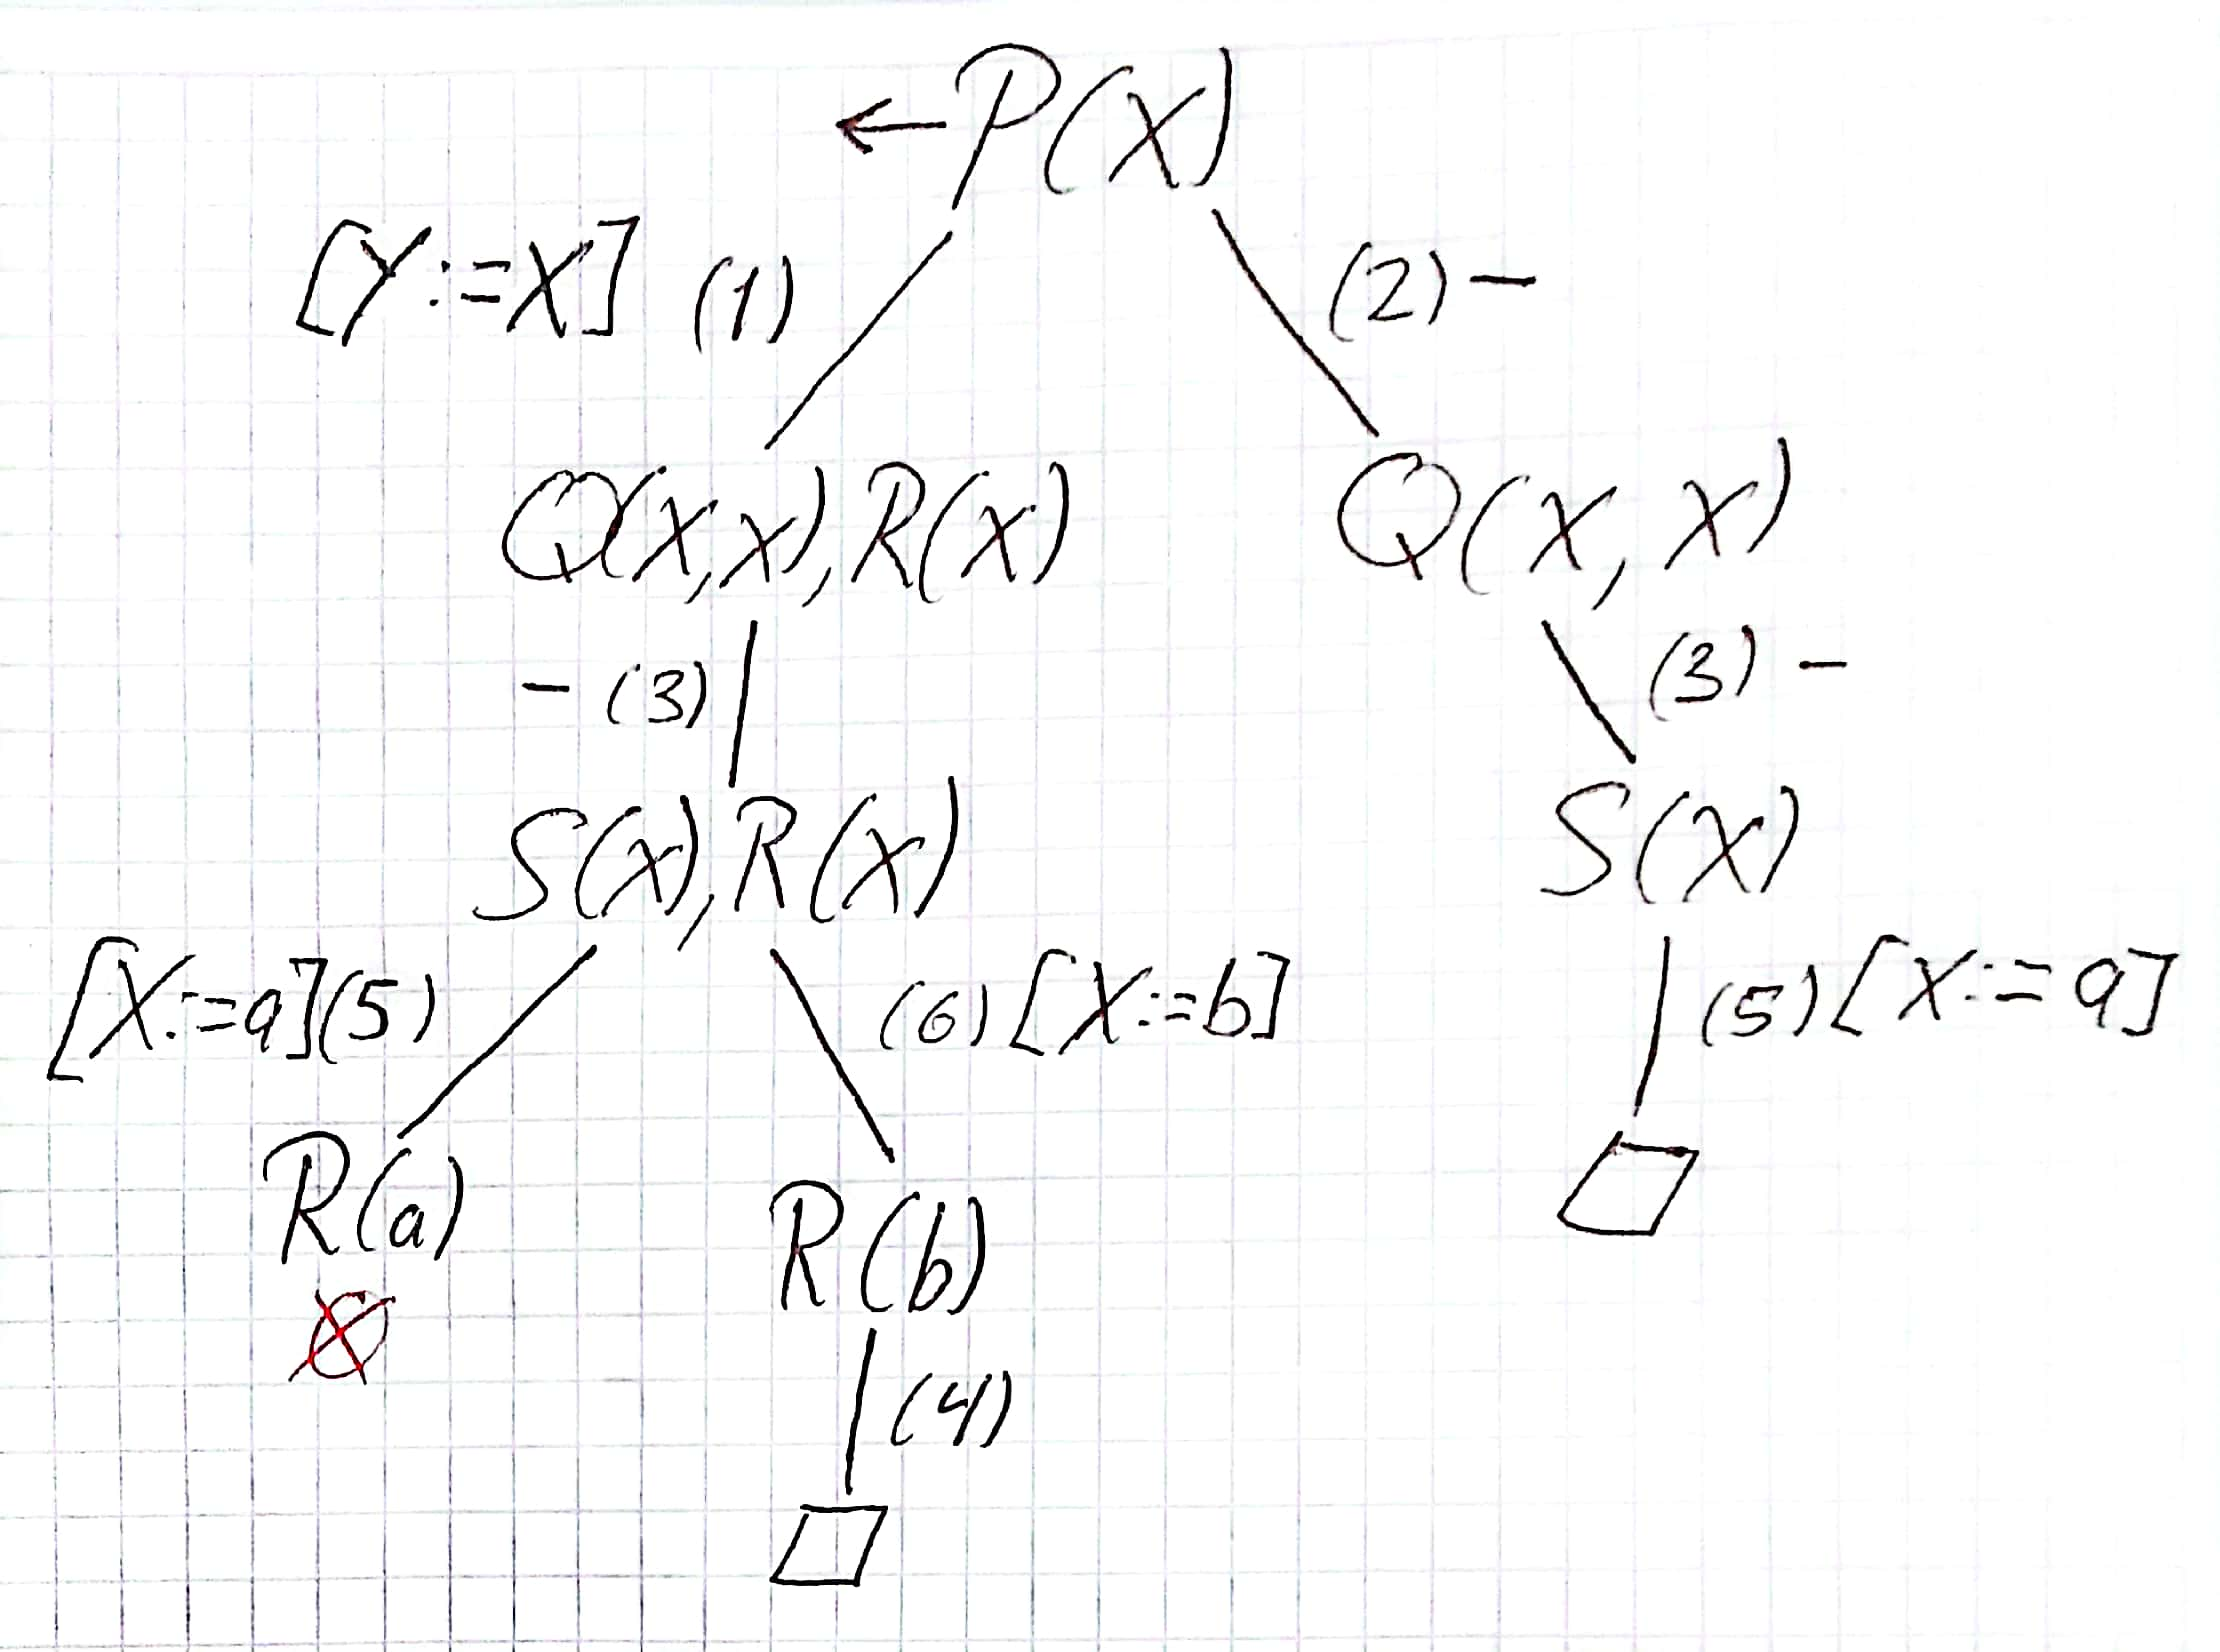
\includegraphics[width=\textwidth,height=0.54\textheight,keepaspectratio]{tree.png}
  \end{center}
  
  Como podemos ver, el árbol SLD obtenido a partir de la meta $\dmp P(X)$ bajo la regla de cómputo de \textsc{Prolog} nos da dos refutaciones posibles:
  \begin{enumerate}[label=\arabic*)]
  \item En la primer cl\'{a}usula vac\'{i}a obtenida, para la rama tenemos la sustitución:
    
    $\theta_1 = [Y:= X, X := b]$
  \item En la segunda cl\'{a}usula vac\'{i}a, para la rama tenemos la sustitución: $\theta_2 = [X := a]$
  \end{enumerate}

  Por lo tanto $[Y := X, X := a]$ y $[X := a]$ son sustituciones de respuesta correcta para el programa con cláusula meta $\dmp P(X)$.
  \bigskip
  
\item (2 pts.) Cónsidere el siguiente programa lógico $\mathcal{P}$:
  \begin{multicols}{2}
\begin{verbatim}
path(X,X,Y).            
path(X,Y, s(Z)):-
         edge(X,A), path(A,Y,Z).
path(X,Y,Z):-
         eps(X,A),path(A,Y,Z).

\end{verbatim}
\begin{verbatim}
edge(a,b).
edge(b,a).
edge(c,d).
edge(d,b).

eps(b,c).
\end{verbatim}
  \end{multicols}
  \vspace{-0.4cm}
  El predicado \verb@edge@ y \verb@eps@ definen la siguiente gráfica $\mathcal{G}$:
  \begin{center}
    \selectlanguage{english}
    \begin{tikzpicture}[->,>=stealth',shorten >=0.7pt,%
        node distance=2.55cm,semithick,
        inner sep=2.5pt,bend angle=45]

      \node[] 		 (A)			                        {\texttt{a}};
      \node[]         (C) [below of=A]                       {\texttt{c}};
      \node[]         (B) [right of=A]                       {\texttt{b}};
      \node[]         (D) [right of=C]                       {\texttt{d}};

      \path 
      (A) edge node {} (B)
      
      (B) edge node {} (A)
      edge node[above] {$\varepsilon$} (C)
      
      (C) edge node {} (D)
      
      (D) edge node {} (B);

    \end{tikzpicture}
    \selectlanguage{spanish}
  \end{center}

  Además, \verb|path(X,Y,Z)| es verdadero syss existe una trayectoria de \verb@X@ a \verb@Y@ en $\mathcal{G}$ donde a lo más \verb@Z@ aristas no etiquetadas con $\epsilon$ fueron usadas a lo largo de la trayectoria. Por ejemplo, \verb@?-path(a,X,s(0))@ da como soluciones \verb@X=a@, \verb@X=b@ y \verb@X=c@. Los números naturales los estamos representando por los símbolos de función \verb@0@ y \verb@s@.

  Dé un árbol SLD para la consulta \verb@?-path(b,b,s(s(0)))@. Los subárboles que \textsc{Prolog} explora después de haber encontrado la segunda solución pueden ser abreviados con ($\ldots$).
  % -- Respuesta --

  \begin{center}
    \hspace{-1.2cm} 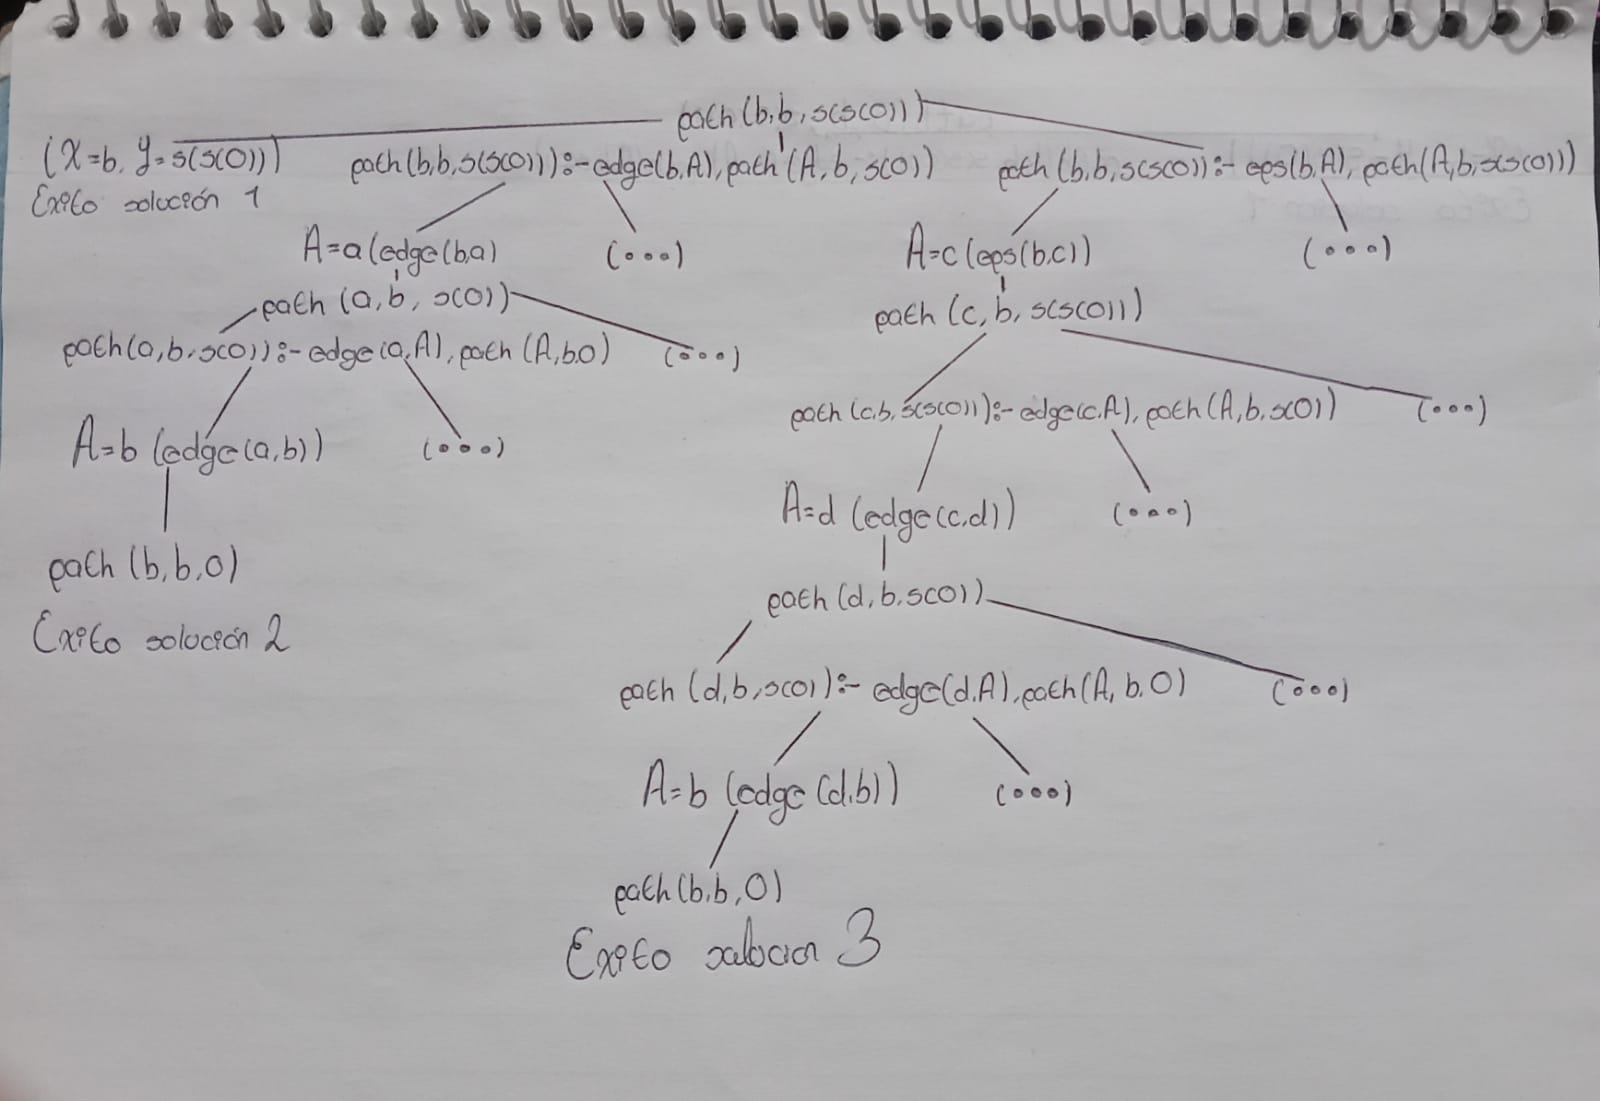
\includegraphics[width=\textwidth,height=0.6\textheight,keepaspectratio]{ejercicio5.png}
  \end{center}
  
\end{enumerate}
\end{document}
